\documentclass{apuntes}
\author{Guillermo Julián Moreno}
\date{13/14 C1}
\title{Estadística I}

\begin{document}

\pagestyle{plain}
\maketitle

\tableofcontents
\newpage

\section{Estadística descriptiva de datos univariantes}

La estadística descriptiva es el conjunto de técnicas para resumir la información proporcionada por una gran masa de datos. El primer objetivo natural es resumir la información que proporcionan esos datos.

\subsection{Estadísticos de tendencia central}
 
\begin{defn}[Media]

\[ \avg{x} = \frac{\sum_{i=1}^n x_i}{n} \]

Es la medida de tendencia central más utilizada. Es bastante sensible a los valores atípicos (\textit{outliers}), observaciones anormalmente grandes que aparecen en el conjunto de datos por errores de transcripción o medición.

\end{defn}

\begin{defn}[Mediana]
Es el valor que divide a los datos en dos mitades, de tal forma que la mitad son menores y la otra mitad mayores que la mediana. 

La mediana se calcula de la siguiente forma: dado un conjunto de datos $\{x_1,\dotsc, x_n\}$, la mediana es $x_{\frac{n+1}{2}}$ si $n$ es impar y  el promedio entre $x_{\frac{n}{2}}$ y $x_{\frac{n}{2} + 1}$.
\end{defn} 

\subsection{Estadísticos de dispersión}

\begin{defn}[Varianza]
\[ \sigma^2 = \frac{1}{n} \sum_{i=1}n \left(x_i - \avg{x}\right)^2 = \frac{1}{n} \sum_{i=1}n x_i^2 - \avg{x}^2 \]
\end{defn}

\begin{defn}[Desviación típica]
\[\sigma = \sqrt{\sigma^2} \]

La desviación típica es la raíz de la varianza.
\end{defn}

\begin{defn}[Cuantil]
Para $p\in (0, 1)$ se llama cuantil $p$ o $q_p$ al valor que deja el $100p \%$ de los datos a la izquierda.
\end{defn}

\begin{defn}[Cuartil]
Los cuartiles son los tres datos que dejan a la izquierda el 25, 50 y 75 por ciento de los datos respectivamente. Es decir:

\begin{itemize}
\item $Q_1 = q_{0.25}$
\item $Q_2 = q_{0.5}$. El cuartil dos es la mediana.
\item $Q_3 = q_{0.75}$
\end{itemize}
\end{defn}

Hay varios métodos para el cálculo de cuantiles. Para hacerlo a mano, podemos usar el siguiente método.

Si el dato en la posición $p(n+1)$ no es un número entero, entones se interpola entre las observaciones ordenadas que están en la posición $\floor{p(n+1)}$ y $\floor{p(n+1)} + 1$ de la siguiente forma: sea $j$ la parte entera de $p(n+1)$ y $m$ la parte decimal. Entonces, \[ q_p = (1-m)x_j + m x_{j+1} \]


\begin{defn}[Coeficiente\IS de asimetría]
\index{Skewness}
El tercer momento con respecto a la media se define como \[ \frac{1}{n}\sum_{i=1}^n\left(x_i-\avg{x}\right)^3 \] que, en su versión adimensional dividimos por $\sigma^3$.
\end{defn}

Al ser una función cúbica, los valores que se alejen mucho de la media tendrán un valor muy alto en valor absoluto (positivo o negativo según se aleje por la derecha o izquierda, respectivamente). Si la distribución de datos es muy asimétrica, los valores más altos no se cancelan con los valores altos del otro lado (porque no hay) y saldrá un valor más alejado de cero.\footnote{Está explicado como el p. culo, ya.}

\subsection{Representación gráfica de datos}

\begin{defn}[Box-plot]
El diagrama de caja o \textit{box-plot}  (imagen \ref{imgCaja}) nos permite visualizar las medidas de dispersión respecto a la mediana. Hay que añadir una nueva medida, el \textbf{rango intercuartílico}\index{Rango!intercuartílico}, la diferencia entre el primer y el tercer cuartil: \[RI = Q_3 - Q_1 \]

\easyimg{DiagramaCaja.png}{Diagrama de caja}{imgCaja}
\end{defn}

\begin{defn}[Histograma]
El histograma se trata de una aproximación discreta a la función de densidad continua $f(t)$ de la variable que estamos midiendo. Es un diagrama de frecuencias que \textit{mantiene la forma} de esa función de densidad. 

Definimos una serie, las marcas de intervalos $a^n_1, \dotsc, a^n_n$, donde $n$ es el número de intervalos y la longitud de cada intervalo  es $h_n = a^n_{j+1} - a^n_j$. Sea el conjunto $\{x_i\}_{i=0,\dotsc,m}$ los datos de nuestra muestra. Entonces, el estimador, la función $\hat{f}_n$, se define de la siguiente forma:

\[ \hat{f}^n(t) = \frac{\card{i \tq x_i \in \left( a_j^n, a_{j+1}^n \right]}}{n h_n} = \frac{\sum_{i=1}^m \ind_{(a_j^n, a_{j+1}^n]} (x_i)}{n h_n} \]

Recordemos que \[ \ind_A (n) = \begin{cases} 1 & n \in A \\ 0 & n \notin A\end{cases}\]

A grandes rasgos, lo que hace en una función es definir un número de intervalos fijos de ancho $h_n$. Al evaluar $\hat{f}^n(t)$ buscamos en qué intervalo cae $t$ y contamos cuántas de nuestras mediciones caen también en ese intervalo.

\easyimg{DensidadAHistograma.png}{El histograma es una aproximación de la función de densidad real en base a la muestra que hemos obtenido.}{lblDensidad}

\end{defn}

\subsubsection{Estimadores núcleo o kernel}

\begin{defn}[Método de ventana móvil][Ventana móvil]
El método de ventana móvil nos da una estimación de la función de densidad en un punto $t$ midiendo los $x_i$ que están en el intervalo de radio $h_n$ centrado en $t$. Matemáticamente:

\[ \hat{f}_n(t) = \frac{1}{n2h_n}\sum_{i=1}^n \ind_{[t-h_n, t+h_n]}(x_i) = \frac{1}{n2h_n}\sum_{i=1}^n \ind_{[-1,1]}\left(\frac{t-x_i}{h_n}\right) \]
\end{defn}

Podemos reemplazar la función $\frac{1}{2}\ind_{[-1, 1]}$ por otra, llamada la función de densidad $K$, kernel o núcleo:

\begin{defn}[Estimador núcleo]
Dada una función de densidad $K$ simétrica, no necesariamente positiva, definimos el estimador kernel como:

\[ \hat{f}_n(t) = \frac{1}{n}\sum_{i=1}^n K_h (t - x_i)  = \frac{1}{nh_n} \sum_{i=1}^n K\left(\frac{t-x_i}{h_n}\right) \]

con $K_h(x) = \frac{1}{h}K(\frac{x}{h})$.
\end{defn}

La elección del núcleo $K$ no afecta especialmente a lo bien aproximada que esté la función de densidad. Sin embargo, sí que influye la selección de la ventana $h_n$ (figura \ref{lblSuavizado}), también llamada \textit{bandwith} en inglés.  Si escogemos una ventana muy pequeña, damos demasiado peso a los datos de nuestra muestra. Si elegimos una ventana muy grande, nuestra muestra pierde importancia y podemos perder información importante.

La elección del $h_n$ más habitual es el que minimiza la distancia $L^2$ entre $\hat{f}$ y $f$, es decir, el parámetro que minimice $\displaystyle\int\left(\hat{f}_h-f\right)^2$. Sin embargo, hay un problema: no sabemos qué es $f$. Hay trucos que imagino que veremos más tarde.

\easyimgw{Suavizado.png}{Los efectos que causa elegir una ventana más grande o más pequeña en el estimador}{lblSuavizado}{1}

Las funciones kernel más usadas son la uniforme, $\frac{1}{2}\ind_{[-1, 1]}$, la gaussiana $\frac{1}{\sqrt{2 \pi}}e^{-\frac{t^2}{2}}$ y la de Epanechnikov, que matemáticamente es la que mejor aproxima $f$.

El estimador kernel $\hat{f}_n(t)$ es la función de densidad de una medida de probabilidad que es la convolución \footnote{Ya aprenderemos en al algún momento de nuestra vida qué narices es una convolución} de dos medidas de probabilidad: una, $K_h(x)$ (el kernel reescalado) y otra que da probabilidad $\frac{1}{n}$ a cada punto de la muestra $\{x_i\}$ (distribución o medida empírica).

\paragraph{Generación de datos del estimador kernel} Supongamos que $K$ es el núcelo gaussiano. Podemos generar datos artificiales de la densidad así:

\[ x_i^0 = x_i^* + h_n Z_i,\; i=1,\dotsc, k \]

donde $x_i^*$ es una observación elegida al azar entre los datos originales y $Z_i$ una observación aleatoria con probabilidad $N(0,1)$. Es decir, lo que hacemos es añadir un dato aleatorio de la muestra y sumamos una pequeña perturbación aleatoria.

\section{Estadística descriptiva de datos bivariantes}

En esta sección estudiaremos dos variables $(X, Y)$ para explorar la relación entre ambas y tratar de inferir si existe una relación funcional para predecir los valores de una variable en función de los de la otra.

\subsection{Representación gráfica}

\begin{defn}[Diagrama\IS de dispersión]
El diagrama de dispersión representa cada variable en función de la otra para que podamos ver la posible relación entre ambas. Ver figura \ref{lblDispersion}.

\easyimg{Dispersion.png}{Diagrama de dispersión}{lblDispersion}
\end{defn} 

\subsection{Regresión}

\begin{defn}[Recta de regresión]

La recta de regresión de $y$ sobre $x$ es la recta de forma $\hat{y} = \hat{a} + \hat{b}x$ que más se aproxima a los datos, minimizando los cuadrados de la distancia: \[ (\hat{a},\hat{b}) =\argmin_{a, b} \sum_{i=1}^n\left(y_i - a - bx_i)\right)^2 \]
\end{defn}

La recta de regresión se calcula obteniendo primero $\hat{b}$:

\[ \hat{b} = \frac{\sigma_{x,y}}{\sigma^2_x} \]

donde \[ \sigma_{x,y} = \frac{1}{n} \left( \sum_{i=1}^n x_i y_i\right)  - \avg{x}\avg{y} \] y después, sabiendo que la recta pasa por el punto $(\avg{x}, \avg{y})$, obtenemos $\hat{a}$ \[ \hat{a} = \avg{y} - \hat{b}\avg{x} \]

El valor $b$ se denomina \textbf{coeficiente de regresión lineal}\index{Regresión lineal!coeficiente de} o parámetro de la regresión. Cada valor $e_i= y_i - \hat{y}_i$ se denomina \textbf{residuo}\index{Residuo}. Hay que notar que

\begin{gather*}
 \sum_{i=1}^n e_i = \sum_{i=1}^n \left(y_i - \hat{a} -\hat{b}x_i \right)= \sum_{i=1}^n\left( y_i - (\avg{y} - \hat{b}\avg{x}) - \hat{b}x_i \right) = \\
 = \sum_{i=1}^n  \left(y_i - \hat{b}x_i\right) - n\avg{y}  + n\hat{b}\avg{x} = n\avg{y} - n \hat{b}\avg{x}- n\avg{y} + n\hat{b}\avg{x} = 0 \end{gather*}

Esta ecuación ($\sum_{i=1}^n e_i = 0$) junto con \[ \sum_{i=1}^n x_i e_1 = 0 \] son las dos restricciones entre los residuos que nos dan la recta.

\begin{defn}[Varianza\IS residual]
La varianza residual $s_R^2$ o $\hat{\sigma}_e^2$ mide, aproximadamente el \textit{error cuadrático} cometido en la aproximación dada por la recta de regresión:

\[ s_R^2 = \hat{\sigma}_e^2 = \frac{1}{n}\sum_{i=1}^n e_i^2 \]
\end{defn}

\begin{defn}[Coeficiente\IS de correlación lineal]
\index{Coeficiente!de Pearson}
El coeficiente de correlación lineal o coeficiente de Pearson

\[ r = \frac{\hat{\sigma}_{x,y}}{\hat{\sigma}_x \hat{\sigma}_y} \] que cumple las siguientes condiciones:

\begin{gather*}
0 ≤ r^2 ≤ 1 \\
\hat{\sigma}_e^2 = \hat{\sigma}_y^2(1-r^2) \\
r = \hat{b}\frac{\hat{\sigma}_x}{\hat{\sigma}_y} 
\end{gather*}

nos indica el grado de ajuste lineal entre las dos variables. Un valor absoluto más cercano a 1 indica una correlación más fuerte. Un valor absoluto cercano a cero indica una correlación débil. El signo, positivo o negativo, indica si la correlación es creciente o decreciente.
\end{defn}


\section{Muestreo aleatorio}

La muestra aleatoria de una cierta v.a. $X$ se denomina como la \textbf{muestra aleatoria} o simplemente \textbf{muestra}.\index{Muestra}

Durante este tema, usaremos conceptos de Probabilidad, que repasaré aquí brevemente porque no me apetece escribir demasiado.

\subsection{Conceptos de probabilidad}

\begin{defn}[Distribución de una v.a.][Distribución]
\[ P_X(B) = P(X \in B) \]
\end{defn}

\begin{defn}[Función de distribución][Distribución!función de]
\[F(t) = P(X ≤ t) \]
\end{defn}

\begin{defn}[Media!de una distribución] También llamada esperanza de X:
\[ E(X) = \int_{-\infty}^\infty F(t)\,dt \]
\end{defn}

\begin{theorem}[Teorema\IS de cambio de espacio de integración] Sea $g$ una función real medible tal que $E(g(X))$ es finita, entonces 

\[ E(g(X)) = \int_\real g(x) \, dF(x) = \int_\real g(x)\, dP(x) \]. 

En particular \[ µ =\int_\real x\, dF(x)  \] y \[ \sigma^2 = \int_\real \left(x - µ\right)^2 \, dF(x) \]
\end{theorem}

\begin{defn}[Momentos] El momento $µ_k$ es la esperanza de X elevado a una potencia de orden $k$. Es el valor esperado de la distancia de orden $k$ con respecto a la media

\[ µ_k = E\left((X-µ)^k\right) \]
\end{defn}

\subsubsection{Distribuciones aleatorias}

Ver apéndice \ref{secDistr} (página \pageref{secDistr}).

\subsubsection{Criterios de convergencia}

Queremos buscar convergencias entre variables aleatorias.

\begin{defn}[Convergencia\IS en distribución]\index{Convergencia!débil} Se dice que $X_n$ converge débilmente o en distribución a $X$ si la función de distribución de $X_n$ $F_n(x)$ tiende a $F(x)$ para todo $x$ punto de continuidad de $F$, donde $F$ y $F_n$ son las funciones de distribución de $X$ y $X_n$ respectivamente.

Esto es equivalente a decir que  \[ \lim_{n\to\infty} P(X_n\in (-\infty, x]) = P(X\in (-\infty, x]) \]

Notación:
\[ X_n  \convdist X \text{ ó }  X_n \xrightarrow[n\to\infty]{w} X \] 
\end{defn}

\begin{defn}[Convergencia\IS en probabilidad] 
Se dice que $X_n$ converge en probabilidad a $X$ si $\forall \epsilon > 0$ se tiene que \[ P(\abs{X_n-X} > \epsilon) \convs 0 \]. Es decir, que para cualquier error que tomemos el error cometido en la aproximación va a tender a cero siempre que tome un $X_n$ suficientemente grande.

Notación: \[ X_n \convprob X \]
\end{defn}

\begin{defn}[Convergencia casi segura] También denotada c.s o a.s en inglés, convergencia en casi todo punto (c.t.p) o convergencia con probabilidad 1. Se dice que $X_n$ converge a $X$ casi seguro si el conjunto de puntos que no son convergentes tiende a ser vacío. Es decir \[ \prob{X_n \convs X} = 1\]

Más estrictamente, la condición se expresa como \[\prob{\omega \in \Omega\tq X_n(\omega) \convs X(\omega)} = 1\]

Notación \[ X_n\convcs X \]
\end{defn}


\begin{theorem}Se puede probar que si $\{X_n\}$ es una sucesión de variables aleatorias y $X$ es variable aleatoria, 

\[ X_n\convcs X \implies X_n \convprob X \implies X_n \convdist X \]
Al contrario no tiene por qué darse.
\end{theorem}


\begin{theorem}[Teorema\IS de Slutsky] Sean $\{X_n\}$, $\{Y_n$ sucesiones de variables aleatorias tales que $X_n\convdist X$, $Y_n\convprob c$ con $c\in\real$ constante. Entonces

\begin{enumerate}
\item $X_n + Y_n \convdist X + c$
\item $X_n \cdot Y_n \convdist X \cdot c$
\item $\dfrac{X_n}{Y_n}\convdist \dfrac{X}{c}$ si $c≠0$.
\end{enumerate}
\end{theorem}

\subsubsection{Desigualdades básicas}

\begin{theorem}[Desigualdad\IS de Markov] Sea $X$ v.a. Entonces, $\forall \epsilon > 0$, \[ \prob{\abs{X} > \epsilon} ≤ \frac{\esp{X}}{\epsilon} \]
\end{theorem}

\begin{theorem}[Desigualdad\IS de Chebichev] En las mismas condiciones del teorema anterior, se cumple que  \[ \prob{\abs{X - \esp{X}} > \epsilon} ≤ \frac{V(X)}{\epsilon^2} \]
\end{theorem}

\appendix

\section{Distribuciones notables}
\label{secDistr}
\includepdf[pages={2-last}, nup=1x3]{Distribuciones.pdf}

\section{Ejercicios}
\section{Tema 1 - Estadística descriptiva}

\begin{problem}[2] Demostrar que \[ \sum_{i=1}^n \left(x_i-\avg{x}\right)^2 = \min_{a\in \real} \sum_{i=1}^n(x_i-a)^2 \]

\solution

Definimos una función \[ g(a) = \sum_{i=1}^n(x_i-a)^2 \], buscamos su derivada \[ g'(a) = -2 \sum_{i=1}^n(x_i-a) \] e igualamos a cero:

\begin{gather*}
-2 \sum_{i=1}^n(x_i-a) = 0 \\
\sum_{i=1}^n x_i - \sum_{i=1}^n a = 0 \\
n \avg{x} = n a \\
\avg{x} = a 
\end{gather*}

Esto quiere decir que la media muestral es el valor que minimiza la distancia con cada uno de los datos de la muestra.
\end{problem}

\begin{problem}[5]Determina si es verdadero o falso:

\ppart Si añadimos 7 a todos los datos de un conjunto, el primer cuartil aumenta en 7 unidades y el rango intercuartílico no cambia.

\ppart Si todos los datos de un conjunto se multiplican por -2, la desviación típica se dobla.

\ppart Al multiplicar por tres todos los datos de un conjunto, el coeficiente de asimetría no varía

\ppart Si el coeficiente de correlación entre dos variables vale -0.8, los valores por debajo del
promedio de una variable están asociados con valores por debajo del promedio de la otra.

\ppart Si $\forall i\,y_i<x_i$ entonces el coeficiente de correlación es negativo.

\ppart Al restar una unidad a cada dato de un conjunto, la desviación típica siempre disminuye.

\ppart Si a un conjunto de datos con media $\gx$ se le añade un nuevo dato que coincide con $\gx$, la
media no cambia y la desviación típica disminuye.

\solution 

\spart Falso. Añadir siete a todos los datos es una traslación, así que la distribución de los datos no cambia. El rango intercuartílico se mantiene y el cuantil también.

\spart Teniendo en cuenta que si multiplicamos todos los datos del conjunto por $-2$ la media también se multiplica por $-2$, y sustituyendo en la fórmula de la varianza:

\[ \sigma' = \sqrt{\frac{1}{n} \sum_{i=1}n (-2x_i)^2 - (-2\avg{x})^2} = \sqrt{\frac{1}{n} \sum_{i=1}4\left(n x_i^2 - \avg{x}^2\right)} = \sqrt{4\sigma^2} = 2\sigma \]

Por lo tanto, la desviación típica sí se dobla.

\spart Usando los cálculos del apartado anterior vemos que la varianza se multiplica por cuatro.

\spart Efectivamente: cambiar el signo haría una reflexión de los datos sobre el eje Y y la asimetría estaría orientada hacia el lado contrario. 

\spart  Teniendo en cuenta que si multiplicamos todos los datos del conjunto por $3$ la media también se multiplica por $3$

El coeficiente de asimetría se calcula:

\[\frac{1}{n} \sum_{i=1}^n (x_i-\gx)^3\]

Sustituyendo en la fórmula del coeficiente de asimetría

\[\frac{1}{n} \sum_{i=1}^n (3x_i - 3\gx)^3 = \frac{1}{n} \sum_{i=1}^n 3^3 (x_i-\gx)^3 = 27 \cdot \frac{1}{n} \sum_{i=1}^n (x-\gx)^3\]

Por lo tanto el coeficiente de asimetría sí varía.

\spart No lo se, pero me la jugaría a falso, porque puede haber un dato más o menos atípico.

\spart Falso. 2 variables pueden tener una correlación creciente aunque $y_i<x_i$.

\spart Falso. La desviación típica se mantiene (los datos siguen estando "igual de separados")

\spart Verdadero. Al hacer el cálculo de la media no varía (en la fórmula del ejercicio 2 se puede comprobar que si añadimos un $x_i=\gx$ el sumatorio de la derecha queda igual) y la desviación típica disminuye.

\end{problem}

\begin{problem}[7]
Relaciona los histogramas con los boxplot
\solution
Fijándose en los intervalos entre los que se mueven los datos es la forma más fácil.

\[\begin{array}{cc}
1 \to 2\\
2 \to 1\\
3 \to 3
\end{array}\]

\end{problem}

\begin{problem}[8]
Del diagrama de dispersión presentado se pregunta:

\ppart ¿Existe alguna relación?

\ppart ¿Hay algún dato atípico?

\ppart De los 3 valores siguientes: $0.01, 0.83, -0,73$ ¿cuál crees que podría corresponder al coeficiente de correlación?

\solution

\spart Parece que sí.

\spart Bastante obvio que sí

\spart 0.83. Es una correlación positiva (creo) y están demasiado correlacionadas como para tener coeficiente $0.01$

\end{problem}

\begin{problem}[10]
¿Qué valor tiene que tomar $x$ para que el coeficiente de correlación sea 1?

\ppart $A = \{(1,1),(2,3),(2,3),(4,x)\}$
\ppart $B = \{(1,1),(2,3),(3,4),(4,x)\}$

\solution

Para que el coeficiente de correlación sea exactamente 1, los puntos tienen que estar en la misma recta. Buscamos el $x$ que cumpla eso.

\spart $x=6$

\spart Imposible (porque los 3 puntos dados no están alineados)

\end{problem}

\section{Tema 2 - Muestreo aleatorio}

\begin{problem}[1] Se desea estimar el momento de orden 4, $\alpha_3 = \esp{X^3}$ en una v.a. $X$ con distirbución exponencial de parámetro 2, es decir, la función de distribución de $X$ es $F(t) = \prob{X ≤ t} = 1 - e^{-2t}$ para $t≥0$. Definir un estimador natural para $\alpha_3$ y calcular su error cuadrático medio.

\solution

Usando el criterio de \textit{plugin}, podríamos definir el estimador \[ \hat{\alpha}_3 = \int_\real x^3\,d\fd_n(x) \]. 

Calculamos ahora el error cuadrático medio:

\begin{gather*}
\ECM (\hat{\alpha}_3) = \esp{\hat{\alpha}_3 - \alpha_3}^2 = \esp{(\hat{\alpha}_3 - \esp{\hat{\alpha}_3} + \esp{\hat{\alpha}_3} - \alpha_3) ^2} = \\
 \underbrace{\esp{(\hat{\alpha_3} - \esp{\hat{\alpha_3}})^2}}_{(a)}+ \underbrace{\left(\esp{\hat{\alpha_3}} - \alpha_3\right)^2}_{(b)} + \underbrace{2 \cdot \esp{ (\esp{\hat{\alpha_3}}- \alpha_3)\cdot(\hat{\alpha}_3 - \esp{\hat{\alpha_3}})}}_{(c)} 
\end{gather*}

Calculamos (b) que es el sesgo:

\[ \sesgo (\hat{\alpha}_3) = \esp{\hat{\alpha}_3} - \alpha_3 = \alpha_3 - \alpha_3 = 0 \]

Como el sesgo es $0$, tenemos que (c) es también 0. Solo nos queda calcular a, que es la varianza:

\[ \var{\hat{\alpha}_3} = \var{\frac{1}{n}\sum X_i^3 } = \frac{1}{n^2}\var{\sum X_i^3} = \frac{1}{n^2}\sum \var{X_i^3} = \frac{\var{X^3}}{n} \]

y, teniendo en cuenta el enunciado,

\[ \var{X^3} = \esp{X^6} - \esp{X^3}^2 = \frac{6!}{2^6} - \left(\frac{3!}{2^3}\right)^2 = \frac{171}{16} \]

y por lo tanto

\[ \ECM (\hat{\alpha}_3) = \frac{171}{16n} = O\left(\frac{1}{n}\right) \convs 0 \]

donde lo que más nos importa es la convergencia a cero, que indica que cuanto más muestras tenemos mejor será el estimador.

\end{problem}

\begin{problem}[2] Supongamos que la muestra tiene tamaño $n=50$ y que la distribución de las $X_i$ es una $N(4,1)$. 

\ppart Obtener, utilizando la desigualdad de Chebichev, una cota superior para la probabilidad $\prob{\abs{\avg{X} - 4} > 0.3}$.

\ppart Calcula exactamente $\prob{\abs{\avg{X} - 4} > 0.3}$ utilizando la distribución de $X_i$. 

\solution
\spart

Como la media es cuatro, la desigualdad de Checbichev nos da una cota de 

\[ \frac{\var{\avg{x}}}{0.3^2} = \frac{\var{X}}{n \cdot 0.3^2} \simeq 0.22 \]


\spart

Normalizamos

\[ Z = \frac{\avg{X} - 4}{\frac{1}{\sqrt{50}}} ~ N(0,1) \]

y calculamos.

\[ \prob{\abs{\avg{X} - 4} > 0.3} = \prob{\abs{Z} > \frac{0.3}{\frac{1}{\sqrt{50}}}} = 2 \cdot \prob{Z > 2.12} = 0.038 \]

\end{problem}

\begin{problem}[4] Denotemos por 

\[ C_n = \int_\real \left(\fd_n(t) - F(t)\right)^2 \, dF(t) \]

la llamada discrepancia de Cramer-Von Mises entre $\fd_n$ y $F$. \ppart ¿Converge a cero casi seguro esta discrepancia?

\ppart Calcular la distribución asintótica de la sucesión $D_n = \sqrt{n}\left(\fd_n(t) - F(t)\right)$ para un valor fijo $t\in\real$.

\solution
\spart 
\[ C_n = \int_\real \left(\fd_n(t) - F(t)\right)^2 \, dF(t) = \int_\real \left(\fd_n(t) - F(t)\right)^2 f(t) \, dt \]

Como por el teorema de Glivenko-Cantelli (\ref{thmGlivenko}) tenemos que 

\[ \fd_n(t) - F(t) ≤ \sup_t \abs{\fd_n(t) - F(t)} = \md{\fd_n - F}_\infty \]

entonces 

\[ \int_\real \left(\fd_n(t) - F(t)\right)^2 f(t) \, dt ≤  \md{\fd_n - F}_\infty^2 \int_\real f(t) \,dt = \md{\fd_n - F}_\infty^2 \]

Igualmente por Glivenko-Cantelli, 

\[ \md{\fd_n - F}_\infty^2 \convcs 0  \qed \]

\spart

Para calcular la distirbución asintótica de \[ D_n = \sqrt{n}\left(\fd_n(t) - F(t)\right) \] usamos el Teorema Central del Límite (\ref{thmCentral}). Necesitamos algo que se asemeje a una media muestral, y de hecho

\[ \fd_n(t) = \frac{1}{n} \sum_{i=1}^n \ind_{(-\infty, t]} (X_i) = \frac{1}{n} \sum_{i=1}^n Y_i = \avg{Y} \]

Por otra parte, $Y = \ind_{(-\infty, t]}(X)$ y por lo tanto \[ \esp{Y} = \esp{\ind_{(-\infty, t]}(X)} = \prob{X ≤ t} = F(t) \]

Ya podemos aplicar el TCL, pero nos falta saber cuál es la desviación típica de $Y$. Como es una distribución de Bernoulli 

\[ \mathbb{V}(Y) = p(1-p) = F(t)(1-F(t)) \]

y por lo tanto 

\[ D_n \convdist N\left(0, \sqrt{F(t)(1-F(t))}\right) \]
\end{problem}

\begin{problem}[5] Sea $X$ una v.a. cuya función de densidad depende de un parámetro desconocido $\theta \in \real$, concretamente \[ f(x;\theta) = \frac{1}{\pi}\frac{1}{1+(x-\theta)^2} \] para $x\in \real$. Comprobar que $\theta$ coincide con la mediana y la moda de $X$ pero que la media $\esp{X}$ no está definida.

Diseñar un experimento de simulación en R, tomando algún valor concreto de $\theta$, orientado a comprobar cómo se comportan la mediana muestral y la media muestral como estimadores de $\theta$: mientras la mediana muestral se acerca al verdadero valor de $\theta$ al aumentar $N$, la media muestral oscila fuertemente y no se acerca a $\theta$ aunque se aumente el tamaño muestral $n$.

\solution Viendo la función, vemos que es simétrica con respecto al eje $x= \theta$. Por lo tanto, el punto que deja a izquierda y derecha la misma probablidad, la mediana, es precisamente $\theta$. 

De la misma forma, la moda es el valor máximo de la distribución, que se ve claramente que ocurre cuando $x=\theta$.
\end{problem}

\begin{problem}[6]
Se extrae una muestra aleatoria de tama~no n = 600 de una v.a. cuya desviación típica es $\sigma = 3$.
Calcular aproximadamente la probabilidad \[\prob{\abs{\gor{X} - \mu} < 0.1}\]
\solution
Tenemos 2 posibilidades: Tipificar o con Chebichev.

Con Chebichev me da negativo... 

Tipificando: \[Z = \frac{\gor{X} - \mu}{\frac{\sigma}{\sqrt{n}}} \sim N(0,1)\]

Entonces:

\[\prob{\abs{\gor{X} - \mu} < 0.1} = 1- \prob{\abs{\gor{X} - \mu} > 0.1} = 1 - \prob{\abs{Z} > \frac{0.1\sqrt{n}}{\sigma}} = 0.59\] 

(Recordamos que $\var{\gor{X}} = \frac{\var{X}}{\sqrt{n}}$ y que $\esp{\gor{X}} = \mu = \esp{X}$)

\end{problem}

\begin{problem}[7] Sea $X$ una v.a con distribución absolutamente continua. Sea $F$ la correspondiente función de distribución y $f = F'$ continua en todo punto la función de densidad. para $r\in \{1,\dotsc,n\}$, denotemos por $X_{(r)}$ el $r$-simo estadístico ordenado de una muestra de tamaño $n$ extraída de $X$. Calcular la función de distirbución y la de densidad de la v.a. $X_{(r)}$.

\solution

Por definición

\[ F_{X_{(r)}} (x) = \prob{X_{(r)} ≤ x }\]

que es la probabilidad que al menos $r$ elementos de la muestra sean menores o iguales que $x$. Luego la probabilidad es igual a

\begin{gather*}
\sum_{j=r}^n \prob{\text{exactamente j observaciones de la muestra son ≤ x}} =  \\
= \sum_{j=r}^n \prob{B(n, F(x)) = j} = \sum_{j=r}^n \comb{n}{j}F(x)^j \left(1 - F(x)\right)^{n-j}
\end{gather*}

Ahora sólo falta calcular la densidad de $X_{(r)}$, y la obtenemos derivando

\begin{gather*}
 f_{X_{(r)}} (x) = \\
 = \sum_{j=r}^n \left(\comb{n}{j}j(F(x)^{j-1}(1-F(x))^{n-j}f(x) - (F(x))^j(n-j)(1-F(x))^{n-j-1} f(x)\right) = \\
 = \sum_{j=r}^n \comb{n}{j} j(F(x)^{j-1}(1-F(x))^{n-j}f(x)  - \sum_{j=r}^n\comb{n}{j} (F(x))^j(n-j)(1-F(x))^{n-j-1} f(x) = \\
 = \comb{n}{r} r(F(x))^{r-1} (1-F(x))^{n-1}f(x) + \sum_{j=r+1}^n \comb{n}{j}j(F(x))^{j-1} f(x) (1-F(x))^{n-j} \\
 \quad \quad - \sum_{j=r}^n\comb{n}{j}(n-j)(F(x))^j (1-F(x))^{n-j-1}f(x) = \\
 n\comb{n-1}{r-1}(F(x))^{r-1} (1-F(x))^{n-r} f(x)    +   \sum_{l=r}^{n-1}n\comb{n-1}{l}(F(x))^l (1-F(x))^{n-l-1} f(x) \\
 \quad\quad -  \sum_{j=r}^{n-1}n\comb{n-1}{j}(F(x))^j (1-F(x))^{n-j-1} f(x)
\end{gather*} 

Los dos últimos términos se cancelan y nos queda que 

\[ f_{X_{(r)}} (x) = n\comb{n-1}{r-1}(F(x))^{r-1} (1-F(x))^{n-r} f(x) \]

Consideremos los dos casos particulares del mínimo y máximo de la muestra. Con el mínimo, $r=1$ y entonces

\[ F_{X_{(1)}} (x)= \prob{X_{(1)} ≤ x} = \sum_{j=1}^n\comb{n}{j}(F(x))^j(1-F(x))^{n-j} = 1 - (1-F(x))^n \]

En el caso del máximo:

\[ F_{X_{(n)}} (x) = \prob{X_{(n)} ≤ x } = (F(x))^n \]

\end{problem}

\begin{problem}[8] Sea $\hat{f}_n$ un estimador kernel de la densidad basado en un núcleo $K$ que es una función de densidad con media finita. Comprobar que, en general, $\hat{f}_n(t)$ es un estimador sesgado de $f(t)$ en el sentido de que \textbf{no} se tiene $\esp{\hat{f}_n(t)} = f(t)$ para todo $t$ y para toda densidad $f$.

\solution

\begin{gather*}
\esp{\hat{f}_n(t)} = \esp{\frac{1}{nh}\sum_{i=1}^n K \left(\frac{t-X_i}{h}\right)} = \\
= \frac{1}{nh}\sum_{i=1}^n \esp{K\left(\frac{t-X_i}{h}\right)} = \frac{1}{h} \esp{K\left(\frac{t-X}{h}\right)} = \\
= \frac{1}{h} \int_\real K \left(\frac{t-x}{h}\right) f(x) \,dx = 
\end{gather*}

Haciendo un cambio de variable $x = t-hz$, $dx = -h\,dz$, los límites se invierten,

\[ = \frac{1}{h} \int_{-\infty}^\infty K \left(\frac{t-x}{h}\right) f(x) \,d(x)  = \frac{-1}{h} \int_\infty^{-\infty} K(z) f(t-hz) h \,dz  = \int_{-\infty}^\infty Kz f(t-hz)\,dz \]

Ahora buscamos calcular el sesgo:

\[ \text{sesgo}\,(\hat{f}_n(t)) = \esp{\hat{f}_n(t)} - f(t) = \]

Usando que $K$ es función de densidad y que $\int K = 1$, nos queda

\begin{gather*}
 = \int_{-\infty}^\infty K(z) f(t-hz)\,dz - \int_{-\infty}^\infty K(z) f(t)\, dz = \\
 = \int_{-\infty}^\infty K(z) \left[f(t-hz)-f(t)\right]\,dz =\\
 = hf'(t)\int_{-\infty}^\infty zK(z)\,dz + \frac{1}{2} h^2 f''(t) \int_{-\infty}^\infty z^2K(z)\,dz + \frac{1}{6}h^3 f'''(t) \int_{-\infty}^\infty z^3K(z)\,dz + \dotsb  
\end{gather*}

al hacer el desarrollo de Taylor. Como $K$ es una función simétrica, las integrales con índice impar (con $z=1, 3,\dotsc$) se anulan. Sin embargo, el segundo término no lo hace. Por lo tanto, el sesgo de un estimador kernel \textbf{no es nunca cero}. 

El sesgo del estimador kernel depende de $h$ (el parámetro de suavizado o \textit{bandwith}) en potencias pares. Por eso, se toma de manera tal que $h\convs 0$ y entonces $\text{sesgo}\,\hat{f}_n(t) \convs 0$ pero manteniendo un equilibrio para que la varianza también sea pequeña y no tengamos picos en el histograma (ver sección \ref{secEst}).

\end{problem}
\section{Tema 3 - Estimación puntual paramétrica}


\begin{problem}[2]
Supongamos que $X$ mide el error cometido en la medici'on de una magnitud. $X$ es una v.a. normal de media 0 y varianza $\theta$. 	
\[X\leadsto N(0,\sqrt{\theta}), \theta>0, \Theta = (0,\infty)\]

Se desea estimar $\theta$ a partir de una muestra.

\ppart Calcular el estimador de máxima verosimilitud $T_n$.

\ppart Probar que $T_n$ es insesgado y eficiente.

\ppart Estudiar la distribución asintótica de $T_n$.
\solution
\spart Buscamos el máximo de la función de verosimilitud
\[L_n(\theta;X_1,...,X_n) = \prod_{i=1}^n f(x_i;\theta) = \frac{1}{\sqrt{2\pi}^{\frac{n}{2}}\theta^{\frac{n}{2}}} e ^ {-\frac{1}{2\theta} \sum x_i^2}\]

El máximo de la función de verosimilitud será también el máximo de la logverosimilitud

\[logL_n(\theta) = \frac{n}{2}\cdot log(2\pi) - \frac{n}{2}log(\theta) - \frac{1}{2\theta} \sum x_i^2\]

Para ello derivamos e igualamos a 0.

\[\dpa{}{\theta} logL_n(\theta) = -\frac{n}{2\theta} + \frac{1}{2\theta^2}\sum x_i^2  = 0\]

\[\frac{1}{2}\left( - \frac{n}{\theta} + \frac{\sum x_i^2}{\theta^2}\right) = 0 \implies T_n = e.m.v.(\theta) = \frac{1}{n}\sum x_i^2\]


\spart $\esp[\theta]{T_n} = \esp[\theta]{\frac{1}{n}\sum x_i^2} = \esp[\theta]{X^2} = \theta$

Nos tenemos que dar cuenta de que $\var{X} = \esp{X^2} - \esp{X}^2$. En este caso $\esp{X} = \mu = 0$ por lo que $\esp{X^2} = \theta$ por hipótesis.
Vamos a calcular la información de fisher para comprobar si el estimador es eficiente o no.

\[ log f(x;\theta) = \frac{-1}{2}log(2\pi)-\frac{1}{2}log(\theta) - \frac{1}{2\theta}X^2\]
Derivamos:
\[\dpa{}{\theta} log f(x;\theta) = -\frac{1}{2\theta} + \frac{1}{2\theta^2}X^2\]
Elegimos derivar otra vez o elevar al cuadrado (2 alternativas para calcularlo).

En este caso vamos a elevar al cuadrado:

\[\dpa{}{\theta}logf(X;\theta) = \frac{1}{4\theta^2} \left( 1+\frac{X^4}{\theta^2} - 2\frac{X^2}{\theta}\right)\]

Entonces la información de fisher será:

\[I(\theta) = \esp[\theta]{\frac{1}{4\theta^2} \left( 1+\frac{X^4}{\theta^2} - 2\frac{X^2}{\theta}\right)} = \frac{1}{4\theta^2} \left( 1+\frac{\esp[\theta]{X^4}}{\theta^2} - 2\frac{\esp[\theta]{X^2}}{\theta}\right)\]

Aplicamos por hipótesis: $\esp[\theta]{X^4} = 3\theta^2$

\[I(\theta) = \frac{1}{4\theta^2} \left(1+\frac{3\theta^2}{\theta^2} - 2 \frac{\theta}{\theta}\right) = \frac{1}{2\theta^2}\]

Vamos a calcular \[\var[\theta]{T_n} = \var[\theta]{\frac{1}{n}\sum x_i^2} = \frac{1}{n^2}\sum \var[\theta]{x_i^2} = \frac{n}{n^2} \var[\theta]{X^2} =\]
\[ \frac{1}{n}\left(\esp[\theta]{X^4} - \esp[\theta]{X^2}\right) = \frac{1}{n}(3\theta^2-\theta^2) = \frac{2\theta^2}{n} = \frac{1}{nI(\theta)}\]

Como la varianza coincide con la cota de Frécher-Cramer-Rao entonces podemos decir que es un estimador eficiente.

Los siguientes pasos para comprobar lo bueno que es el estimador son: \begin{itemize}
\item $T_n$ asintóticamente normal.
\item $T_n$ es consistente casi seguro.
\end{itemize}

\spart Vamos a estudiar la distribución asintótica:

\[\sqrt{n}(T_n-\theta) \convs[d] N(0,\sigma(\theta))\]

Llamando $Y_i = X_i^2 \implies \esp[\theta]{Y} = \esp[\theta]{X^2} = \theta$

Entonces por el TCL (Teorema Central del Límite): \[\displaystyle \sqrt{n}(\hat{Y} - \esp[\theta]{Y}) \convs[d] N(0,\sqrt{\var{Y}})\]

Donde $\var{Y} = \var[\theta]{X^2} = \esp{(X^2)^2} - \esp{X^2}^2 = 3\theta^2 - \theta^2 = 2\theta^2$
\end{problem}



\begin{problem}[3] Se dispone de un gran lote de piezas producidas en una cadena de montaje. Denotemos por $p$ la proporción de piezas defectuosas en ese lote. Supongamos que se seleccionan al azar sucesivamente (con reemplazamiento) piezas del lote hasta que se encuentra una defectuosa. Sea $X$ la variable aleatoria que indica el número de la extracción en la que aparece la primera pieza defectuosa.

\ppart Calcular $\prob{X=k}$ para $k=1,2,\dotsc$ Obtener el estimador de $p$ por el método de los momentos, a partir de una muestra $X_1,\dotsc , X_n$.

\ppart Obtener el estimador de $p$ por el método de máxima verosimilitud. Calcular su distribución asintótica.
\solution
\spart
La probabilidad sigue una distribución geométrica de parámetro $p$:

\[ \prob{X=k} = (1-p)^{k-1}p \]

\spart Calculamos la función de verosimilitud:

\[ L(p;x_1,\dotsc,x_n) = \prod_{i=1}^n f(x_i;p) = \prod_{i=1}^n (1-p)^{x_i - 1}p = (1-p)^{\sum_{i=1}^n x_i - 1} p^n \]

Tomamos logaritmos

\[ \log L(p) = \log(1-p) \left(\sum_{i=1}^n x_i - 1\right) + n\log p \]

y derivando

\[ \deriv{}{p} \log L(p) = \frac{-1}{1-p} \left(\sum_{i=1}^n x_i - 1\right)  + \frac{n}{p} \] 

\[n(1-p) = p \sum_{i=1}^n x_i - 1 \dimplies p = \frac{n}{n + \displaystyle \sum_{i=1}^n (x_i-1)} = T_n\]

El $emv(p) = \displaystyle\frac{1}{1 + \gx}$.

Vamos a calcular su distribución asintótica. Para ello llamamos $Y = \displaystyle \frac{1}{1+x}$.

Calculamos $\gor{Y} = \displaystyle\frac{1}{1+\gx}$ (esto está medio inventado).

Suponiendo que ese resultado es correcto, por el TCL tenemos:

\[\sqrt{n} \left(T_n - \frac{1}{1+\gx}\right) \convs[d] N\left(0,\sqrt{\var{X}}\right)\]

Entiendo que esto no termina de contestar a la distribución asintótica del estimador, con lo que "despejando" $T_n$ obtenemos:

\[T_n \convs[d] N\left(\frac{1}{1+\gx} , \sqrt{n}\sqrt{ \var{X}}\right)\]

\end{problem}

\begin{problem}[4]
Estudiar si es eficiente el estimador de máxima verosimilitud de una poisson.
\solution


\[P(X==k) = e^{-\lambda} \frac{\lambda^{k}}{k!}\]

El cálculo dle estimador de máxima verosimilitud se hizo en clase llegando a $\lambda = \gor{x}$ (\ref{ejEmvPoisson}).

Para ver si es eficiente vemos si es su varianza es igual a la cota de FCR. Necesitamos la información de Fisher para comprobar eso.

Para calcular la información de fisher derivamos el logaritmo de la densidad

\[log f(\lambda;x_1,...,x_n) = -\lambda + k log(\lambda) - \sum log...\]

\[\dpa{}{\lambda} log f (\lambda;x_1,...,x_n) = - 1 + \frac{x_k}{\lambda} + 0\]

Para calcular la información de Fisher podemos volver a derivar o elevar al cuadrado. Elegimos volver a derivar

\[\dpa{^2}{^2\lambda} log f (\lambda;x_1,...,x_n) = -\frac{x_k^2}{\lambda^2}\]

Entonces tenemos que \[I(\lambda) = \esp{-\dpa{^2}{^2\lambda} log f (\lambda;x_1,...,x_n)} = \esp{\frac{x_k}{\lambda^2}} = \frac{1}{\lambda^2}\esp{X} = \frac{1}{\lambda}\]

La cota de FCR será entonces $\displaystyle\frac{1}{n\frac{1}{\lambda}} = \frac{\lambda}{n}$.

Calculamos la varianza:

\[\var{\lambda} = \var{\gx} = \frac{\var{x}}{n} = \frac{\lambda}{n}\]

Como tenemos la igualdad podemos afirmar que \textbf{si} es un estimador eficiente.
\end{problem}

\begin{problem}[5]
Distribución de Rayleigh, cuya función de densidad es:
\[f(x;\theta) = \frac{x}{\theta^2} e^{\frac{-x^2}{2\theta^2}} \mathbb{I}_{[0,\infty)} (x), \theta > 0\]

\ppart Calcular el estimador de máxima verosimilitud (e.m.v.)

\ppart Calcular la consistencia.

\ppart ¿Es asintóticamente normal?

\solution

\spart

\[L_n(\theta;x_1,...,x_n) = \frac{x_1 \cdot ... \cdot x_n}{\theta^2} e^{\frac{-1}{2\theta^2} \sum_{i=1}^n x_i^2}\]
\[log L_n(\theta) = \sum log x_i - 2nlog\theta -\frac{1}{2\theta^2}\sum x_i^2\]
\[\dpa log L_n(\theta) = \frac{1}{\theta} \left(-2n+\frac{1}{\theta^2}\sum x_i^2\right) = 0\]
\[\implies \hat{\theta}^2 = \frac{\sum x_i^2}{2n} \implies \hat{\theta} emv(\theta) = (\frac{\sum x_i^2}{2n}^2\]

Estimador razonable porque $E(x^2) = V(x) + E(x) = 2\theta^2 \dimplies \theta^2 = \frac{1}{2} E(x^2)$

Buscamos ahora el estimador $\tilde\theta$ por el \textbf{método de los momentos}

\[ \esp[\theta]{X}= \theta\sqrt{\frac{\pi}{2}} = \avg{X} \] 

y entonces el estimador es \[\tilde{\theta} = \avg{X}\sqrt{\frac{2}{\pi}} \]

\spart

\textbf{Consistencia:} $\hat{\theta}^2 = \frac{1}{2} \gor{Y}, Y_i = X_i^2$

Por la ley fuerte de los grandes números (\ref{thmGrandes}) sabemos que: $\gor{Y} \convs[cs] E_{\theta}(Y) = E_{\theta}(X^2) = 2\theta^2$

Vamos a aplicar el teorema de Slutsky.

Sea $g(x) = \sqrt{\frac{1}{2}x}$ definida sobre $[0,\infty)$.

Teorema de Slutsky (\ref{thmSlutsky}) $\implies g\left(\gor{Y}\right) = \sqrt{\frac{1}{2} \frac{\sum x_i^2}{n}} \convcs g(E_{\theta}) = \sqrt{\frac{1}{2}\theta^2} = \theta \implies $ El e.m.v. de $\theta$, $\hat{\theta}$ es consistente c.s.


\spart

Queremos aplicar el método delta:

\[\sqrt{n}(\hat{\theta} - \theta) = \sqrt{n}\left(g\left(\gor{Y}\right) - g\left(E(Y)\right)\right) \convs[d]N(0,\abs{g'(E(Y))}\sqrt{V(Y)}\]

\[E_{\theta}(Y) = E_{\theta} (X^2) = 2\theta^2\]
\[V_{\theta}(Y) = E(X^4) - E^2(X^2) = 8\theta^4-4\theta^4 = 4\theta^4\]

Entonces tenemos que $g'(E(Y)) = \displaystyle \frac{1}{2\sqrt{2E(Y)}} = \frac{1}{4\theta}$.

Con esta información completamos:  

\[\sqrt{n}(\hat{\theta} - \theta) \convs[d] N\left(0,\sqrt{\frac{1}{2\theta}}\right)\]

Buscamos ahora la convergencia asintótica del estimador por el método de los momentos:

\[ \sqrt{n}(\tilde\theta-\theta) = \sqrt{n}\left(\avg{X}\frac{2}{\pi}  - \esp{X}\frac{2}{\pi}\right) = \sqrt{\frac{2}{\pi}}\sqrt{n}(\avg{X}-\esp{X}) \]

que, por el TCL (\ref{thmCentral})

\[ \sqrt{\frac{2}{\pi}}\sqrt{n}(\avg{X}-\esp{X})  \convdist  \sqrt{\frac{2}{\pi}}N\left(0,\theta\sqrt{\frac{4-\pi}{2}}\right) = N\left(0,\theta\sqrt{\frac{4-\pi}{\pi}}\right) \]

y por lo tanto es efectivamente asintóticamente normal.

\end{problem}


\begin{problem}[8] Sea $X \sim N(µ,\sqrt{\theta})$. Estamos interesados en la estimación de $\theta$ basados en muestras $X_1,\dotsc,X_n$ de tamaño $n$. Calcular la cota de Fréchet-Cramer-Rao (\ref{thmCotaFCR}) para estimadores insesgados.

\solution

La cota FCR es \[ \frac{1}{n I(\theta)} \]

Podíamos calcular la información de Fisher como

\[ I(\theta) = \esp{\left(\dpa{}{\theta}\log f(X;\theta)\right)^2} = - \esp{\frac{∂^2}{∂\theta^2}\log f(X;\theta)} \]

Usaremos la segunda expresión. Calculamos primero el logaritmo:

\[ \log f(X;\theta) = \frac{-1}{2}\log 2\pi - \frac{1}{2}\log \theta - \frac{1}{2\theta}(x-µ)^2 \]

y derivamos dos veces

\begin{gather*}
 \dpa{}{\theta} \log f(X;\theta) = \log f(X;\theta) = -\frac{1}{2\theta} + \frac{1}{2\theta^2}(x-µ)^2 \\
 \frac{∂^2}{∂\theta^2} \log f(X;\theta) = \frac{1}{2\theta^2} - \frac{2}{2\theta^3} (x-µ)^2 = \frac{1}{\theta^2} \left(\frac{1}{2} - \frac{1}{\theta}(x-µ)^2\right) 
 \end{gather*}
 
 Calculamos ahora la esperanza:
 
 \[ \esp{\frac{1}{\theta^2} \left(\frac{1}{2} - \frac{1}{\theta}(x-µ)^2\right) } = -\frac{1}{\theta^2}\left(\frac{1}{2} - \frac{1}{\theta} \underbrace{\esp{X-µ}^2}_{\theta}\right) = \frac{1}{2\theta^2} \]
 
 y por lo tanto la cota FCR vale $\dfrac{2\theta^2}{n}$, el valor mínimo.

\end{problem}

\begin{problem}[9] Sea $X_1,\dotsc,X_n$ una muestra de una v.a. con función de densidad 

\[ f(x;\theta) = \theta x^{\theta - 1} \]

Sea  \[ T_n(X_1,\dotsc,X_n) = \frac{-1}{n}\sum_{i=1}^n\log X_i \]

\ppart Probar que \[\esp[\theta]{T_n} = \frac{1}{\theta};\; \var[\theta]{T_n} = \frac{1}{n\theta^2} \]
\ppart ¿Es eficiente $T_n$ como estimador de $\frac{1}{\theta}$?

\solution

\spart

\[ \esp[\theta]{T_n} = -\esp[\theta]{\log X} = - \int_0^1 \log x \theta x ^{\theta-1}\,dx = \frac{1}{\theta} \]

Calculamos ahora la varianza:

\begin{gather*}
\var[\theta]{T_n} = \frac{1}{n\theta^2} = \esp[\theta]{T_n^2} - \esp[\theta]{T_n}^2 = \frac{\var[\theta]{\log X}}{n} = \\
= \esp[\theta]{\log^2 X} - \esp[\theta]{\log X}^2 = \frac{1}{\theta^2}
\end{gather*}

\end{problem}


\begin{problem}[11]
\footnote{Este ejercicio es del parcial del año pasado}

ashkjdf
\solution

$X\leadsto Unif[0,\theta]$
Con \[ f(x) = \displaystyle\left\{\begin{array}{cc}
\frac{1}{\theta} & 0\leq x \leq \theta\\
0 & x \notin [0,\theta]
\end{array}\right.\]

Vamos a calcular la función de distribución:

\[F_{\theta} (x) = \mathbb{P}_{\theta}\{X\leq x\} = \int_{-infty}^x f_{\theta}(t)dt = \int_0^x \frac{1}{\theta} dt = \frac{x}{\theta} \ si 0\leq x \leq \theta\]

\[F_{\theta} = \left\{\begin{array}{cc}
\frac{x}{\theta} & 0\leq x \leq \theta\\
0 & x \notin [0,\theta]
\end{array}\right.\]

Nos piden dibujar las funciones. 



Vamos a calcular \[L_n(\theta;x_i) = \prod_{i=1}^n f_{\theta} (x_i) = \left\{\begin{array}{cc}
\left(\frac{1}{\theta}\right)^n & \forall x_i \in [0,\theta]\\
0 & \exists x_i\notin [0,\theta]
\end{array}\right.\]

Calculamos la $logL_n$ que nos piden dibujarla:

\[logL_n(\theta) = \left\{\begin{array}{cc}
-nlog(\theta) & si \ max(\{x_i\})\leq \theta\\
0 & si \ no
\end{array}\right.\]
Dibujoo!

\[\hat{\theta_n} = e.m.v.(\theta) = max\left(L_n(\theta)\right)\]

También vale tomando el logaritmo:

\[\hat{\theta}_n = e.m.v. (\theta) = arg\ mas logL_n(\theta) = max\{x_i\}\]
porque \[ logLn(\theta) = \displaystyle\left\{\begin{array}{cc}
-nlog(\theta) & max\{x_i\} \leq \theta\\
-\infty & si \ no
\end{array}\right.\]
\end{problem}

\section{Tema 4 - Intervalos de confianza}

\begin{problem}[1 y 2]

\ppart Representa un estimador de la función de densidad de la v.a. X = cantidad de contaminación por mercurio (en p.p.m.) en los peces capturados en los ríos norteamericanos Lumber y Wacamaw (ver fichero Datos-mercurio.txt). Comparar esta densidad estimada con la densidad normal de igual media y desviación típica (representada en la misma gráfica). En vista de las dos funciones dirías que la función de densidad de X es aproximadamente normal?

\ppart Obtener un intervalo de confianza de nivel 0.95 para la media de X.

\ppart Se puede considerar fiable este intervalo a pesar de la posible no-normalidad de X?

\ppart Qué tamaño muestral habrá que tomar para estimar la contaminación media con un error máximo de 0.06?
\solution
Solucionado por Amparo, descargable \href{http://www.uam.es/personal_pdi/ciencias/abaillo/MatEstI/T4DatosMercurio.pdf}{aquí}.

\end{problem}

\begin{problem}[3]

\ppart Representa en un mismo gráfico las densidades de las distribuciones $\chi^2_k $ con k = 4,8,20,30.

\ppart $X \sim \gamma(5,10)$. Calcular $\mathbb{P}\{X\leq 3\}$

\ppart Sea $Y \sim \chi_{200}^2$. Calcular $\mathbb{P}\{Y\leq 3\}$

\solution
\spart
El código R utilizado para generar las gráficas es:

\begin{verbatim}
> x = seq(0,20,length.out=1000)
> d1=dchisq(x,df=4)
> d2=dchisq(x,df=8)
> d3=dchisq(x,df=10)
> d4=dchisq(x,df=20)
> plot(x,d1,type='l')
> lines(x,d2,type='l',col='blue')
> lines(x,d3,type='l',col='green')
> lines(x,d4,type='l',col='red')
\end{verbatim}

\begin{center}
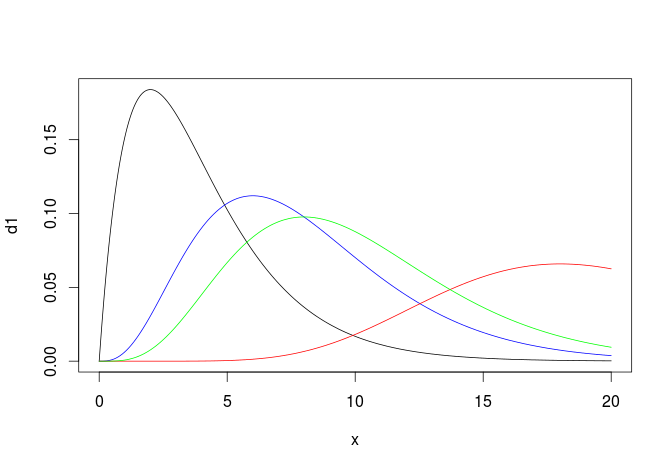
\includegraphics[width=1\textwidth]{Chicuadrado.png}
\label{Ejercicio 4}
\end{center}

\spart
Vamos a usar el resultado visto en clase:
Si $X\sim \gamma(a,p)$ entonces tenemos que 
\[cX \sim \gamma(c\cdot a, p)\]

En este caso, tomando $c=10$ tenemos:

\[\mathbb{P}\{10X\leq 30\} = \mathbb{P}\{\chi^2_{20 }\leq 30\}  \]

Tenemos varias opciontes. Una de ellas es ir a R y calcularlo con el comando \emph{pchisq(30,20)} = 0.93

Y la otra es irse a las tablas y vemos que $\mathbb{P}\{\chi^2_{20} \leq 30\} \simeq 0.93$

\spart Sea $Y \sim \chi_{200}^2$ 

Podemos hacerlo en R directamente y nos da $\mathbb{P}\{Y\leq 3\} = 10 ^{-141}$

A mano, aplicamos el T.C.L, que dice:
\[\sqrt{n}(\gor{X} - \mu) \convs[d] N(0,\sigma)  \]

Entonces tenemos: $\gor{X} \sim N\left(\esp{X},\displaystyle \sqrt{\frac{\var{X}}{n}}\right)$

Donde $\esp{X} = \esp{Z^2} = \var{Z} = 1$ y $\var{X} = \var{Z^2} = \var{\chi_1^2} = 2$

Con lo que:
\[\gor{X} \sim N\left(1,\frac{1}{10}\right)\]

Sustituyendo y estandarizando:

\[
\mathbb{P}\{\gor{X}\leq\frac{3}{20} \} \simeq \mathbb{P} \{Z\leq \frac{\frac{3}{200} - 1}{\frac{1}{10}} \} = \mathbb{P} \{Z\leq -9.85\} = 3 \cdot 10^{-23}
\]

Una diferencia bastante distinta a lo que decía R. Tras un debate entre Miguel y Amparo de 10 minutos no se ha llegado a ninguna conclusión.
\end{problem}

\begin{problem}[4]
\ppart Utilizando el fichero Datos-lipidos.txt, estima, mediante un intervalo de confianza de nivel
0.95, la proporción de pacientes que tienen una concentración de colesterol superior o igual a
220 mg/dl. ¿Qué tamaço muestral habrá que usar para tener una probabilidad aproximada de 0.95 de no cometer un error mayor que 0.01 en la estimación de esta proporción?

\ppart
\solution
Solucionado por Amprao, descargable 
\href{http://www.uam.es/personal_pdi/ciencias/abaillo/MatEstI/T4DatosLipidos.pdf}{aqui}
\end{problem}
\begin{problem}[5] Sea una v.a. con función de densidad $f(x;\theta) = \theta x^{-(\theta) + 1}\ind_{[1,\infty)} $

\ppart Obtener el e.m.v.

\ppart Obtener su distribución asintótica

\ppart Calcular la cantidad pivotal aproximada y, a partir de ella, un intervalo de confianza de nivel aproximada $1-\alpha$ para $\theta$
\solution
\spart \[\dpa{logL(\theta)}{\theta} = 0 \implies e.m.v.(\theta) = \frac{1}{\gor{Y}}\]
donde $Y = log X_i$

\spart Posibles caminos:

a) $\hat{\theta} \convs[d] $¿?

b) \[\sqrt{n}(\hat{\theta} - \theta) \convs[d] N\left(0,?\right)\]

La primera opción es algo difusa y la segunda es mucho más concreta y mejor.

Tenemos que examinar la expresión $\sqrt{n}(\hat{\theta} - \theta)$
Tenemos 2 posibilidades con las que calcular este tipo de cosas (T.C.L) y método delta (que es el que emplearemos a continuación)

\[\mu = \esp{X}; \sigma = \var{X}\]
\[\sqrt{n}\left(g(\gor{X}) - g(u)\right) \convs N(0,\abs{g'(u)} \sigma\]

Aplicando el método delta:

\[
\sqrt{n}(\hat{\theta} - \theta) = \sqrt{ n}\left(g(\gor{y})-g(\esp{Y})\right)\convs[d] N\left(0,\underbrace{\abs{g'\left(\frac{1}{\theta}\right)}}_{\theta^2} \sqrt{\var{Y}}\right) = N(0,\theta)
\]

Peeero... hay que tener cuidado con que $\theta = g(\esp{Y})$ porque sino no podemos aplicar el método delta.

\[
\var{Y} = \esp{Y^2} - \esp{^2 Y} = \underbrace{\int_1^2 (log\,x)^2 \theta x^{-(\theta + 1)}dx}_{\displaystyle\frac{2}{\theta}} - \frac{1}{\theta^2} = \theta{1}{\theta^2}
\]

\spart
La cantidad pivotal les un estadístico que depende de la muestra y del parámetro desconocido (del que estamos calculando el intervalo) y cuya distribución, al menos asintóticamente) es totalmente conocida.

En el apartado b) hemos encontrado la distribución asintótica para poder construir la cantidad pivotal.

Tipificamos el resultado anterior para evitar que la distribución depende del parámetro desconocido.

\[
\frac{1}{\theta} \sqrt{n}(\hat{\theta} - \theta)  = 
\sqrt{n} \left(\frac{\hat{\theta}}{\theta} - 1 \right) = \mathbb{Q}(\theta;X_1,...,X_N)
\]

Esta es nuestra cantidad pivotal, que depende de la muestra (por el $\hat{\theta}$) y depende del parámetro.

\[1-\alpha  = \mathbb{P} = \{q_1(\alpha) \leq \mathbb{Q}(\theta;X_1,...,X_N) \leq q_2 (\alpha)\}\]


El despejar se deja como ejercicio para el lector.

\end{problem}

\begin{problem}[6]
Sea $\sample$ una muestra de una v.a. uniforme en el interalo $[0,θ]$ con $0 < θ < 1$. Obtener una cantidad pivotal para $θ$ a partir del emv. Usando esta cantidad pivotal construye un intervalo de confianza para $θ$ de nivel prefijado $1-α$.

\solution

El e.m.v es \[ emv (θ) = \hat{θ} = \max X_i \] La cantidad pivotal para $θ = Q(θ; \sample)$

\[ F_{X_{(n)}} (x) = \prob{\hat{θ}_n ≤ x} = \prob{X_{(n)} ≤ x} = \prod_{i=1}^{n} \prob{X_i ≤ x} = \begin{cases}
0& x<0 \\
\left( \frac{x}{θ} \right)^n & 0≤x≤θ \\
1 & x > 1
\end{cases}\]

Tomo $Q(θ; \sample ) = \dfrac{X_{(n)}}{θ} = \dfrac{\hat{\theta}}{n}$, que es válido como cantidad pivotal porque \[ \prob{Q≤x} = \prob{\frac{X_{(n)}}{θ} ≤ x} = \begin{cases}
0 & x<0 \\
x^n & 0≤x≤θ \\
1 & x > 1
\end{cases} \]

Tenemos que elegir dos valores $q_1, q_2$ de tal forma que 

\[ 1- α = \prob{q_1(α) ≤ Q(θ;\sample) ≤ q_2(α)} \]

¿Cómo elegirlos? Queremos buscar que la longitud del intervalo de confianza $IC_{1-α}(θ) = \left(\dfrac{\hat{θ}_n}{q_2},\dfrac{\hat{θ}_n}{q_1}\right)$ sea mínima. Calculamos esa longitud:

\[ \text{len IC} = \hat{θ}_n\left(\frac{1}{q_1}-\frac{1}{q_2}\right)=\hat{θ}_n \left(\frac{q_2-q_1}{q_1q_2}\right) \]

Es decir, tenemos que buscar que $q_1-q_2$ sea más pequeño y además tienen que ser lo mayores posible. Por lo tanto, la elección óptima es 

\[ q_2 = 1,\;q_1=α^{1/n} \]

\end{problem}

\begin{problem}[7] Construye tres intervalos de confianza asintóticos diferentes para el parámetro $λ$ de una distribución de Poisson usando los tres métodos siguientes:

\ppart Utiliza el comportamiento asintótico de la media muestral, estima de forma consistente la varianza y aplica el teorema de Slutsky.

\ppart Igual que el anterior, pero sin estimar la varianza

\ppart Aplicando el método delta para \textit{estabilizar la varianza}, es decir, buscando una función $g$ tal que $\sqrt{n}(g(\avg{X}) - g(λ))\convdist N(0,1)$.

\solution

\spart El TCL (\ref{thmCentral}) nos dice que

\[ \sqrt{n}\frac{\avg{X} - λ}{\sqrt{λ}} \convdist N(0,1) \]

Entonces tenemos que 
\begin{equation}
 1-α = \prob{-z_{α/2}≤\sqrt{n}\frac{\avg{X} - λ}{\sqrt{λ}} ≤ z_{α/2}} \label{eqEj7}
 \end{equation}

Sustituyo $λ$ en el denominador por una estimación consistente $\hat{λ}\convs[P, c.s]λ$:

\[ \sqrt{n}\frac{\avg{X} - λ}{\sqrt{\hat{λ}}} \convdist N(0,1) \]

Como sabemos que $λ=\esp{X}$, tomamos la media muestral como el estimador: $\hat{λ} = \avg{X}$. La convergencia nos queda entonces como


\[ \sqrt{n}\frac{\avg{X} - λ}{\sqrt{\avg{X}}} \convdist N(0,1) \]

y por lo tanto tomamos $ \sqrt{n}\dfrac{\avg{X} - λ}{\sqrt{\avg{X}}}$ como nuestra cantidad pivotal. Despejamos ahora en (\ref{eqEj7}):

\[ \prob{\avg{X} - z_{α/2} \sqrt{\frac{\avg{X}}{n}} 
	≤ λ
	≤ \avg{X} + z_{α/2} \sqrt{\frac{\avg{X}}{n}}}
	\]
	
\spart Partimos de nuevo de (\ref{eqEj7}), pero no tenemos que estimar $λ$. Esta ecuación es equivalente a 

\[ \prob{n\frac{(\avg{X}-λ)^2}{λ} ≤ z_{α/2}^2} \]

De ahí sólo tenemos que despejar $λ$ para hallar nuestro intervalo de confianza.

\spart Tenemos que buscar que se satisfaga la ecuación \[ \sqrt{n}(g(\avg{X}) - g(λ))\convdist N(0,1) \]

Sin embargo, el método delta (\ref{defMetDelta}) nos dice algo distinto:

\[ \sqrt{n}(g(\avg{X}) - g(λ))\convdist N(0,\abs{g'(μ)}\sqrt{\var{X}}) \]

Entonces tenemos que 

\[ \abs{g'(λ)}\sqrt{λ} = 1 \implies g'(λ) = \frac{1}{\sqrt{λ}} \]

e integrando vemos que $g(λ) = 2\sqrt{λ} $.
\end{problem}

\begin{problem}[8]
\ppart Se desea evaluar aproximadamente, por el \textit{método de Montecarlo}, la integral 

\[ p = \int_0^1f(x)\,dx \] 

de una función continua $\appl{f}{[0,1]}{[0,1]}$. Para ello se generan 500 observaciones independientes $(X_i,Y_i)$ con $i=1,\dotsc,500$ con distribución uniforme en el cuadrado $[0,1]×[0,1]$ y se estima $p$ mediante

\[ \hat{p} = \sum_{i=1}^{500} \frac{Z_i}{500} \]

donde la v.a. $Z_i$ vale 1 si $Y_i≤f(X_i)$ y $0$ en caso contrario. ¿Qué distribución tienen las $Z_i$? Suponiendo que, en una muestra concreta hemos obtenido $\sum_{i=1}^{500} z_i = 255$, obtener un intervalo de confianza de nivel $0.99$ para la correspondiente estimación de $p$.

\solution

\spart La v.a. sigue una distribución de Bernoulli, de tal forma que

\begin{equation} \prob{Z=1}=\prob{Y ≤ f(X)} \label{eqEj8} \end{equation}

La distribución de densidad de la v.a. $(X_i, Y_i)$ es 

\[ f(x,y) = \begin{cases}
1 & (x,y) ∈ [0,1]×[0,1] \\
0 & \text{en otro caso}
\end{cases} \]

Aplicando esto en $(\ref{eqEj8})$

\[ \prob{Z=1} = \prob{(X,Y) ∈ \{(x,y)\tq y ≤ f(x) \}} = \int_0^1\int_0^{f(x)} \,dy\,dx = \int_0^1f(x)\,dx = p \]

y llegamos a la forma de estimar la integral que queríamos. 

Vamos a contruir el intervalo de confianza de nuvel $0.99$.

\[IC_{0.99} (p) = \left(\gor{z} \pm Z_{0.005}\sqrt{\frac{\gor{z}(1-\gor{\gz})}{500}}\right) = \left(\hat{p} \pm 2575 \sqrt{\frac{\hat{p}(1-\hat{p})}{500}}) \right) = (0.45\pm 0.057)\]


\spart En este caso sabemos el valor de \[p = \int_0^1 x^2dx = \frac{1}{3}\]
Buscamos un $n$ que cumpla: \[z_{0.005} \sqrt{\frac{\frac{1}{3}\cdot\frac{2}{3}}{n}} \implies n > 14734.72\]

\end{problem}

\begin{problem}[9]
Sea X una v.a. con distribución normal de media $\mu$ y variandza $\theta$. Estamos interesados en la estimación de $\theta$ basados en muestras $X_1,...,X_n$. Si $s^2$ denota la cuasivarianza muestras, calcular $\var{s^2}$ y compararla con la cota de Fréchet-Cramer-Rao obtenida en la relación 3 de problemas.
\solution

Comentarios previos: Sabemos que $s^2$ es un estimador insesgado de \[\var{X} = \frac{1}{n-1} \sum_{i=1}^n (X_i - \gor{X})^2\]

Vamos a calcular $\var{s^2}$

Posibilidades:
\begin{itemize}
\item Aunque es un poco largo\[
\var{s^2} = \esp{s^2}-\left[\esp{s^2}\right]^2
\]

\item Si $X\sim N(\mu,\sigma)$ entonces \[\frac{(n-1)s^2}{\sigma^2} \sim \chi_{n-1}^2\]
\end{itemize}

Vamos a utilizar la segunda opción (es un resultado que pondría una referencia pero no se donde está)

\[
\var{s^2} = \var{\frac{n-1}{\sigma^2}s^2\cdot\frac{\sigma^2}{n-1}} = \frac{\sigma^4}{(n-1)^2} \var{\frac{n-1}{s^2}} s^2 = \frac{\theta^2}{(n-1)^2}2(n-1) = \frac{2\theta^2}{n-1} \]

$s^2$ por lo tanto no es eficiente $\left( \text{porque la Cota de FCR es: } \displaystyle\frac{2\theta}{n}\right)$ Por ser $\theta$ la varianza de una $N(\mu,\sigma)$, de la que nos sabemos de memoria la cota de FCR.


\end{problem}

\section{Tema 5 - Contraste de hipótesis}
\subsection{Hoja 5A}

\begin{problem}[1] En octubre de 2007 el periódico \textit{The New York Times} realizó un muestreo en 20 restaurantes y tiendas de Nueva York con objeto de analizar la variable $X$, que representa el contenido en ppm de metilmercurio en el sushi de atún que se pone a la venta. La media y la cuasi-desviación típica muestrales obtenidas con estas 20 observaciones de $X$ fueron $\avg{x} = 0.794,\, s=0.2953$. Supongamos que $X$ tiene distribución aproximadamente normal.

\ppart ¿Proporcionan estos datos suficiente evidencia estadística a nivel $0.05$ a favor de la hipótesis de que la concentración media de metilmercurio en las raciones de sushi de atún en la población considerada es superior a 0.6 ppm? El p-valor, ¿es menor o mayor que 0.01?

\ppart Obtener, a partir de estos datos, un intervalo de confianza de nivel 0.95 para la concentración media de metilmercurio $μ$ en toda la población. Calcular el mínimo tamaño muestral mínimo que habría que utilizar para, con una probabilidad de 0.95, estimar la concentración media de metilmercurio con un error máximo de 0.06 ppm.

\solution

\spart Empezamos definiendo la hipótesis nula, que será que $μ≤0.6$ ya que queremos una evidencia muy fuerte para rechazar que la concentración suba del nivel mínimo.

La región de rechazo en este caso es 

\[ R = \{ T > t_{19;α} \}\]

donde \[ T = \frac{\avg{x} - 0.6}{0.2953/\sqrt{20}} = 2.938 \]

Por otra parte, $t_{19;α} = 1.729$. Se cumple la condición de la región de rechazo, por lo tanto rechazamos $H_0$. El p-valor del contraste tendrá que ser menor entonces que $0.05$.

Para saber si el p-valor es menor que $0.01$ calculamos $t_{19;0.01}=2.53$. Como sigue siendo menor que $T$, seguimos rechazando $H_0$ y por lo tanto el p-valor del contraste será menor que $0.01$.

Si quisiésemos obtener el p-valor concreto del contraste, buscaríamos el valor de $α$ tal que $ t_{19;α} = 2.938$. En R, obtendríamos este valor con la orden

\begin{verbatim}
> pt(2.938, 19, lower.tail=FALSE)
[1] 0.004221168
\end{verbatim}

El p-valor es por lo tanto $0.004$. Esto quiere decir que la probabilidad de obtener la muestra que hemos conseguido suponiendo que $H_0$ es cierta (esto es, suponiendo que la media de ppm de metilmercurio en el atún es menor que $0.6$) es extremadamente baja, y o bien hemos obtenido una muestra muy, muy extraña o $H_0$ es falsa. Por lo tanto, lo razonable sería rechazar la hipótesis nula y decir que, de media, la concentración de metilmercurio media es mayor que $0.6$.

\spart El intervalo de confianza sería 

\[ IC_{0.95} (μ) = \left(\avg{x}\pm t_{n-1;\frac{α}{2}}\frac{s}{\sqrt{n}} \right) = (0.656, 0.932) \]

Como además $0.6\notin IC_{0.95}(μ)$, rechazaríamos $H_0:\,μ=0.06$ a nivel $α=0.05$.

Para hallar el tamñao muestral mínimo buscamos que 

\[ IC_{0.95}(μ) = (\avg{x} \pm 0.06)\]

Despejando, tenemos que resolver

\[ t_{n-1;0.025}\frac{s}{\sqrt{n}} < 0.06\]

Como no conocemos $s$, lo sustituimos por una aproximación, la cuasivarianza muestral de los 20 restaurantes que teníamos al principio. Además, intuimos que $n$ va a ser grande y por lo tanto $t$ se aproximaría a una distribución normal $Z = N(0,1)$, y por lo tanto

\[ t_{n-1;0.025} ≈ z_{0.025} = 1.96 \]

y entonces $n > 93$.
\end{problem}

\begin{problem}[8] 

\ppart Supongamos que en una determinada población de referencia, formada por adultos sanos, el nivel en sangre de la enzima hepática GGT (gamma-glutamil-transpeptidasa) sigue aproximadamente una distribución normal con media polacional $42 IU/L$ y desviación típica poblacional 13. Calcular aproximadamente el porcentaje de personas en la población que tienen un nivel de GGT superior a 80.

\ppart Supongamos ahora que se selecciona una muestra de 61 personas en otra población formada por bebedores habituales no diagnosticados de alcoholismo y se obtiene una media muestra de 58 IU/L con una desviación típica de 21. ¿Hay suficiente evidencia estadística, al nivel 0.05, para afirmar que la concentración media de GGT en la población de bebedores es mayor que 42?

\solution

Sí.

\end{problem}

\begin{problem}[4] Los niveles en sangre de una hormona denominada FSH están asociados con la fertilidad femenina. Las mujeres que tienen un nivel de FSH "alto" (superior a 10 IU/L) tienen en general más dificultad para concebir que aquellas que tienen niveles bajos de FSH. En un estudio realizado recientemente, se analizó la posible relación entre el grupo sanguíneo y la fertilidad. Para ello se midieron los niveles de FSH en una muestra de 254 mujeres en edad fértil con grupo sanguíneo "O" y resultó que 43 de ellas tenían niveles altos de FSH y, por tanto, podrían tener dificultades para concebir. En otra muestra, independiente de la anterior, de 309 mujeres cuyo grupo sanguíneo no es O, resultó que 27 tenían niveles altos de FSH. 

\ppart ¿Proporcionan estos datos suficiente evidencia estadística, al nivel 0.05, a favor de la hipótesis de que las mujeres con grupo sanguíneo 0 tienen más dificultades para concebir que las que tienen otro grupo sanguíneo?

\ppart Calcular el tamaño muestral necesario para, con probabilidad 0.95, estimar en la población de mujeres del grupo 0 el porcentaje de las que tienen un nivel alto de FSH, con un error máximo de 2 puntos.

\solution

Consideramos la v.a. $X$ que vale $1$ si una mujer del grupo 0 tiene nivel alto de FSH y 0 si no, y que sigue una distribución de Bernoulli con probabilidad $p_1$. Análogamente, definimos la v.a. $Y$ que vale $1$ si una mujer del grupo no 0 tiene nivel alto de FSH y 0 si no, y que sigue una distribución de Bernoulli con probabilidad $p_2$.

Tenemos que 

\begin{gather*}
\sum_{i=1}^{254} x_i = 43 \\
\sum_{i=1}^{309} y_i = 27 
\end{gather*}

\spart Primero tenemos que definir la hipótesis nula:

\[ H_0:\: p_1≤p_2 \]

es decir, que las mujeres con grupo 0 no tienen más dificultad para concebir. Tomamos esto como la hipótesis nula porque es la que aceptamos por defecto, y queremos una evidencia muy fuerte para poder decir que es falsa.

Para construir la región de rechazo, usamos la región del formulario para comparación de proporciones. Usando el TCL, tenemos que si $p_1=p_2=p$ entonces tanto $\avg{X}$ como $\avg{Y}$ van a seguir una distribución normal con $n_i = n_1$ o $n_2$ según sea $X$ ó $Y$

\[ N\left(p, \sqrt{\frac{p(1-p)}{n_i}}\right) \]

y por lo tanto el estadístico del contraste es

\[ Z = \frac{\avg{X} - \avg{Y}}{\sqrt{\avg{p}(1-\avg{p})\left(\frac{1}{n_1}+\frac{1}{n_2}\right)}} \]

siendo $\avg{p}$ un estimador puntual de $p$, y que se calcula como 

\[ \avg{p} = \frac{\sum x_i + \sum y_i}{n_1 + n_2} = \frac{n_1\avg{x} + n_2\avg{y}}{n_1 + n_2} \]

La región de rechazo es

\[ R = \left\{ \avg{x} - \avg{y} > z_{0.05}\sqrt{\avg{p}(1-\avg{p})\left(\frac{1}{n_1}+\frac{1}{n_2}\right)} \right\} \equiv \{ 0.0819 > 0.0460 \} \]

y por lo tanto rechazamos la hipótesis nula al nivel $α=0.05$.

Calculamos ahora el p-valor para tener más datos sobre la hipótesis:

\[ \text{p-valor}\, = \prob{N(0,1) > z} = \dotsb \]

\spart Necesitamos un intervalo de confianza

\[ IC_{0.95}(p_1) = \left(\avg{x} \pm z_0.025\sqrt{\frac{\avg{x}(1-\avg{x}}{n_1}}\right) \]

donde $z_0.025\sqrt{\frac{\avg{x}(1-\avg{x}}{n_1}}$ es el error cometido al estimar $p_1$ con el IC, y que tiene que ser menor que $0.02$. Como no tenemos el valor de $\avg{x}$, lo sustituimos por el valor de la media muestral obtenido en la anterior medición, de tal forma que tenemos que $n_1≥1351$ para obtener la confianza requerida. 

Si quisiésemos ser más conservadores, sustiuiríamos $\avg{x}$ por el valor máximo que podemos obtener, aunque en este caso saldría un tamaño muestral mucho más grande.

\end{problem}

\begin{problem}[5] El gasto telefónico medio bimensual en una muestra de 10 usuarios elegidos al azar en una ciudad ha resultado ser 90 euros y la cuasidesviación típica 11 euros. En otra ciudad se ha tomado, de modo independiente, otra muestra de 12 usuarios y los valores obtenidos para la media y la cuasidesviación típica muestrales han sido, respectivamente, 80 y 10.

\ppart ¿Proporcionan estos datos suficiente evidencia estadística, al nivel 0.05, a favor de la hipótesis  de que el gasto medio en la primera ciudad es más alto que el gasto medio en la segunda? Suponer que las varianzas de las variables que indican los gastos telefónicos en ambas ciudades son iguales. Indicar claramente las restantes suposiciones necesarias para garantizar la validez del procedimiento empleado.

\ppart El p-valor ¿es mayor o menor que 0.01? Razonar la respuesta.

\solution

\spart Definimos las dos variables aleatorias que tenemos: $X$ es el gasto medio bimensual en la primera ciudad, y $Y$ el gasto en la segunda. Tomamos las esperanzas y varianzas:

\begin{gather*}
\esp{X} = μ_1,\;\var{X} = σ_1^2 \\
\esp{Y} = μ_2,\;\var{Y} = σ_2^2 
\end{gather*}

 Definimos la hipótesis nula: $H_0:\, μ_1≤μ_2$, es decir, que el gasto medio en la primera ciudad no es mayor que en la segunda.
 
 Tenemos que suponer que $X$ e $Y$ son normales para poder definir bien el estadístico del contraste. Si usásemos cualquier otra distribución el estadístico del contraste toma una distribución mucho más complicada que no podríamos determinar correctamente. También suponemos que son independientes.                       

La región de rechazo es 

\[ R = \left\{ \avg{x} - \avg{y} > t_{n_1+n_2-2, α} s_p\sqrt{\frac{1}{n_1} + \frac{1}{n_2}}\right\} \] 

Calculando, tenmos que 

\begin{gather*}
\avg{x}-\avg{y} = 10\\
s_p^2 = 109.45 \\
R= \{10 > 7.73 \}
\end{gather*}

y por lo tanto rechazamos la hipótesis nula.

\spart Calculamos la región de rechazo para $α=0.01$:

\[ R= \{10 > 11.32 \} \]

y por lo tanto para nivel $0.01$ no hay evidencia para rechazar $H_0$. Entonces, el p-valor es mayor que $0.01$.

\end{problem}

\begin{problem}[6]
Se realiza un experimento para comparar los incrementos en los niveles plasmáticos de insulina producidos por la ingesta de carne y de pescado. PAra ello se midieron los incrementos (medido esn picomoles por litro) producidos en la concentración de insulina en la sangre de 6 voluntarios, 90 minutos después de comer un bistec de 250 gramos. Dos días más tarde se realizó de nuevo el experimento con las mismas 6 personas, después de consumir un filete de pescado. En la tabla se observan los resultados:

\begin{tabular} {|l|c|c|c|c|c|c|}
\hline
Persona & 1 & 2 & 3 & 4 & 5 & 6\\
\hline
Resultados con la carne: & 109& 106 & 111& 105 & 110 & 108\\
\hline
Resultados con el pescado: & 100& 95& 105& 106& 80& 88\\
\hline
\end{tabular}

\ppart Proporcionan estos datos suficiente estadística a nivel significación 0.05 para afirmar que el incremento medio...?
\solution

\spart 

\paragraph{1)} Definir las variables:
\begin{itemize}
\item $X$ nivel de insulina en 1 voluntario tras la ingesta de carne. Llamamos a $\esp{X} = \mu_1$
\item $Y$ nivel de insulina en \textbf{el mismo} voluntario tras la ingesta de carne. $\esp{Y} = \mu_2$
\end{itemize}

Tenemos que las variables no son independientes (porque son muestras tomadas de los mismo voluntarios). A este tipo de datos le llamamos datos emparejados \index{Datos \IS emparejados}

\paragraph{2) Definir las hipótesis}
\begin{itemize}
\item $H_0: \mu_1 \leq \mu_2$
\item $H_1 : \mu_1>\mu_2$
\end{itemize}

\paragraph{3)} Como tenemos datos emparejados, podemos trabajar más facilmente con la diferencia, es decir, definimos $D=X-Y$ y definimos el contraste (siendo $\esp{D}=\mu$)
\begin{itemize}
\item $\Huge_0 : \mu \leq 0$
\item $H_1: \mu >0$
\end{itemize}

Que es un contraste equivalente.

Además tenemos que $D \sim N(\mu,\sigma)$ 

Suponer que la diferencia es una normal es el procedimiento estándar para datos emparejados. (nos la jugamos, es una hipótesis del problema, que puede ser más o menos razonable. En este caso, lo único que de momento sabemos hacer es suponer que es normal (si no fuera normal, tendríamos que aplciar el TCL (para lo que necesitamos n grande) y con este tamaño muestral (6) no podríamos aplicarlo)

Mirando en la tabla de regiones de rechazo tenemos:
\[R = \left\{\gor{d}> t_{n-1;\alpha} \frac{s_d}{\sqrt{n}}\right\}\]
Donde $\displaystyle \frac{\gor{d}}{s_d/\sqrt{n}}$ es el estadístico del contraste, que sigue una $t_{n-1}$.

De los datos extraemos $\gor{d} = 12.5;s_d=10.97$.

Para $\alpha = 0.05$ calculamos el cualtil correspondiente de la $t$ de Student. Para $\alpha = 0.05$ es 9.02.

De aquí deducimos que sí hay evidencia para rechazar la hipótesis nula (porque  $\displaystyle \frac{\gor{d}}{s_d/\sqrt{n}} > 9.02$).

\spart Tomando $\alpha = 0.01$ no se cumple la condición de rechazo, no pudiendo negar entonces la hipótesis nula.

\spart Es el típico ejercicio mecánico de extraer el tamaño muestral.
\end{problem}

\subsection{Hoja 5B}

\begin{problem}[1] Tenemos una $X \sim \mop{exp}(\theta)$. Queremos contrastar para $\alpha = 0.01$ las dos siguientes hipótesis: $H_0: \theta = 5$ frente a $H_1: \theta = \theta_1$, siendo $\theta_1 > 5$ un valor prefijado.

\ppart Obtener la región crítica del test UMP.

\ppart Calcular la probabilidad de error de tipo II en este test.

\ppart Supongamos que para una determinada muestra, se obtiene $\sum_{i=1}^5 x_i= 5$. ¿Qué decisión habría que adoptar si se utiliza el test construido en a)?
\solution

\spart Ejemplo típico de aplicar el lema de Pearson. Primero comprobamos la propiedad de CVM:

\[\frac{f_n(\sample[x];θ_1)}{f_n(\sample[x];5)} = \left(\frac{θ_1}{5}\right)^n e^{-(θ_1-5)\sum x_i} \]

Efectivamente, la función es monótona.

La región de rechazo del test UMP es, por el lema de Neyman-Pearson (\ref{thmNeymanPearson}), la siguiente:

\[ R^{\ast} = \left\{ \left(\frac{\theta_1}{5}\right)^n e^{(-\theta_1-5)\sum x_i > k_α}\right\}
	 = \left\{\sum x_i < c_{\alpha}\right\} \]
	 
¿Cómo construimos $c_{\alpha}$? Tiene que cumplir $\prob[\theta=5]{\sum x_i < c_{\alpha}} = \alpha$

Como $X$ es una exponencial, tenemos que 

\[ \sum X_i \sim γ(θ;n) \]

y entonces

\[ \prob[θ=5]{R}= \prob{γ(5;n) < c_α} \]

De esta forma, $c_α$ es el cuantil $α$ de la distribución Gamma $γ(5;n)$:

\[ c_α = q_{5,n}(α) \]

\spart Calculamos el error de tipo dos, la probabilidad de aceptar la hipótesis nula cuando es falsa:

\[ \prob[θ_1]{R^c}=1-\prob[θ_1]{R} = 1- \prob[θ_1]{\sum X_1 < q_{5,n}(0,01)} = 1 - \prob{γ(θ_1;n)<q_{5,n}(0,01)} \]

Usando las propiedades de la distribución gamma, tenemos que

\[ γ(θ_1;n) = γ\left(\frac{θ_1}{5}5;n\right) = \frac{5}{θ_1}γ(5;n) \]

y entonces

\[ \prob[θ_1]{R^c} = 1 - \prob{γ(5;n) < \frac{θ_1}{5}q_{5,n}(0,01)}
 	= \prob{γ(5;n)≥ \frac{θ_1}{5}q_{5,n} (0,01)} \] 
 	
Este valor tiende a 0 cuando $θ_1\to∞$.

\spart Nuestra muestra nos da una estimación puntual de $\avg{x} = 1$. Bajo la hipótesis nula, la media de la población nos debería de dar $\frac{1}{5}$. Bajo la hipótesis alternativa, la media debería ser estrictamente menor que $\frac{1}{5}$.

Entonces, hay más evidencia a favor de la hipótesis nula así que esperaríamos aceptarla. Comprobémoslo ahora calculando la región de rechazo.

Tenemos que calcular el cuantil de la distribución Gamma:

\[ q_{5,5}(0.01) = 0.2558 \]

No se satisface la condición de la región de rechazo y por lo tanto no hay evidencia para rechazar la hipótesis nula, tal y como habíamos intuido.
\end{problem}

\begin{problem}[3]
El error que se comete en la medición de una magnitud es una v.a. $X$ cuya función de densidad es 

\[ f(x;θ) = \frac{1}{\sqrt{2πθ}}e^{-\frac{x^2}{2θ}} \]

siendo $θ>0$ un parámetro que se desea estimar. Obtener el test uniformemente más potente de nivel $α$ para contrastar $H_0:\,θ≤θ_0$ frente a $H_1:\,θ$

\solution Tenemos que comprobar primero que el cociente de verosimilitudes es monótono. Para ello cogemos dos valores ya ordenados y calculamos la razón de verosimilitudes:

\[ \frac{f(\sample[x];θ_2)}{f(\sample[x];θ_1)} = \left(\frac{θ_1}{θ_2}\right)^{\frac{n}{2}} e^{-\frac{1}{2}\left(\frac{1}{θ_2}-\frac{1}{θ_1}\right)\sum x_i^2} \]

que sí es una función creciente de $T_n=\sum x_i^2$. Por lo tanto esta es una familia paramétrica CVM (ver definición \ref{defFamCVM}). Aplicando el teorema (\ref{thmNeymanPearson2})

\[ R = \{ T_n > k_α \} \tq \prob[θ_0]{R} = α \] 

¿Cómo resolvemos la expresión de $k_α$?

\[ k_α=θχ_{n;α}^2 \]

\end{problem}

\begin{problem}[5] Sea $X_1,\dotsc, X_{16}$ una muestra de tamaño 16 de una población normal de esperanza $μ$ y varianza $σ^2=1$. Se desea contrastar $H_0:\,μ=0$ frente a $H_1:\,μ≠0$.

\ppart Calcula la región crítica del contraste de razón de verosimilitudes de nivel $α=0.05$. ¿Qué decisión se toma a nivel $α=0.05$ si con 16 datos se ha obtenido una media muestra $\avg{x}=1$?

\ppart Para el contraste anterior, ¿cuál es el valor de la función de potencia evaluada en $μ=0.75$?
\solution

\spart
Calculamos la función de verosimilitud:

\[ f(\sample[x];μ) = \frac{1}{(2π)^{n/2}} e^{-\frac{1}{2}\sum(x_i-μ)^2} \]

Nuestro espacio paramétrico es 
\begin{gather*}
Θ_0 = \{ μ=0 \} \\
Θ = ℝ 
\end{gather*}

Entonces el cociente es 

\[ Λ_n = \frac{f(\sample[x];0)}{f(\sample[x];\avg{x}}
 = e^{-\frac{1}{2}\left(\sum x_i^2 - \sum(x_i-\avg{x})^2\right)} = 
e^{-\frac{1}{2}n\avg{x}^2} \]

La región de rechazo es

\[ R=\{ Λ_n < k_α \} \] 

donde $k_α$ es tal que $\prob[μ=0]{R} = α$. La región de rechazo se puede expresar de forma equivalente

\[ R=\{ -2\log Λ_n > c_α\} = \{ n\avg{x}^2> c_α \} \]

con $c_α$ cumpliendo la misma condición que $k_α$. Es decir

\[ α = \prob[μ=0]{n\avg{X}^2 > c_α} \]

Sabemos que la distribución de una media de normales es también una normal: $\avg{X} \sim N\left(0,\frac{1}{\sqrt{n}}\right)$. De la misma forma $\sqrt{n}\avg{X}^2\sim N(0,1)$ y finalmente $n\avg{x}^2\sim χ_1^2$. Entonces

\[ R=\{ n\avg{x}^2 > χ_{1;α}^2 \]

A nivel $α=0.05$, tenemos que \[ R = \{ 15 > 3.84 \], y por lo tanto rechazamos la hipótesis nula.

\spart Tenemos que

\[ β_n(μ=0.75) = \prob[μ=0.75]{\mathrm{rechazar}\,H_0} = \prob[=0.75]{R} = \prob[μ=0.75]{n\avg{X}^2> χ_{1;α}^2} \] 

Evaluando

\[ n\avg{X}^2 = n(\avg{X}-0.75+0.75)^2 = n(\avg{X}-0.75)^2 + 0.75^2 + 2(\avg{X}-0.75)\cdot 0.75 \]

¿Cómo evaluar esta probabilidad? Hacemos algo raro

\end{problem}





\newpage
\printindex
\end{document}